\documentclass[border=5mm]{standalone}
\usepackage{luamplib}
\usepackage{graphicx}
\mplibtextextlabel{enable}
\begin{document}

    \begin{mplibcode}

        input marly.mp ;

        beginfig(0);
        picture A,B;
        A = TEX("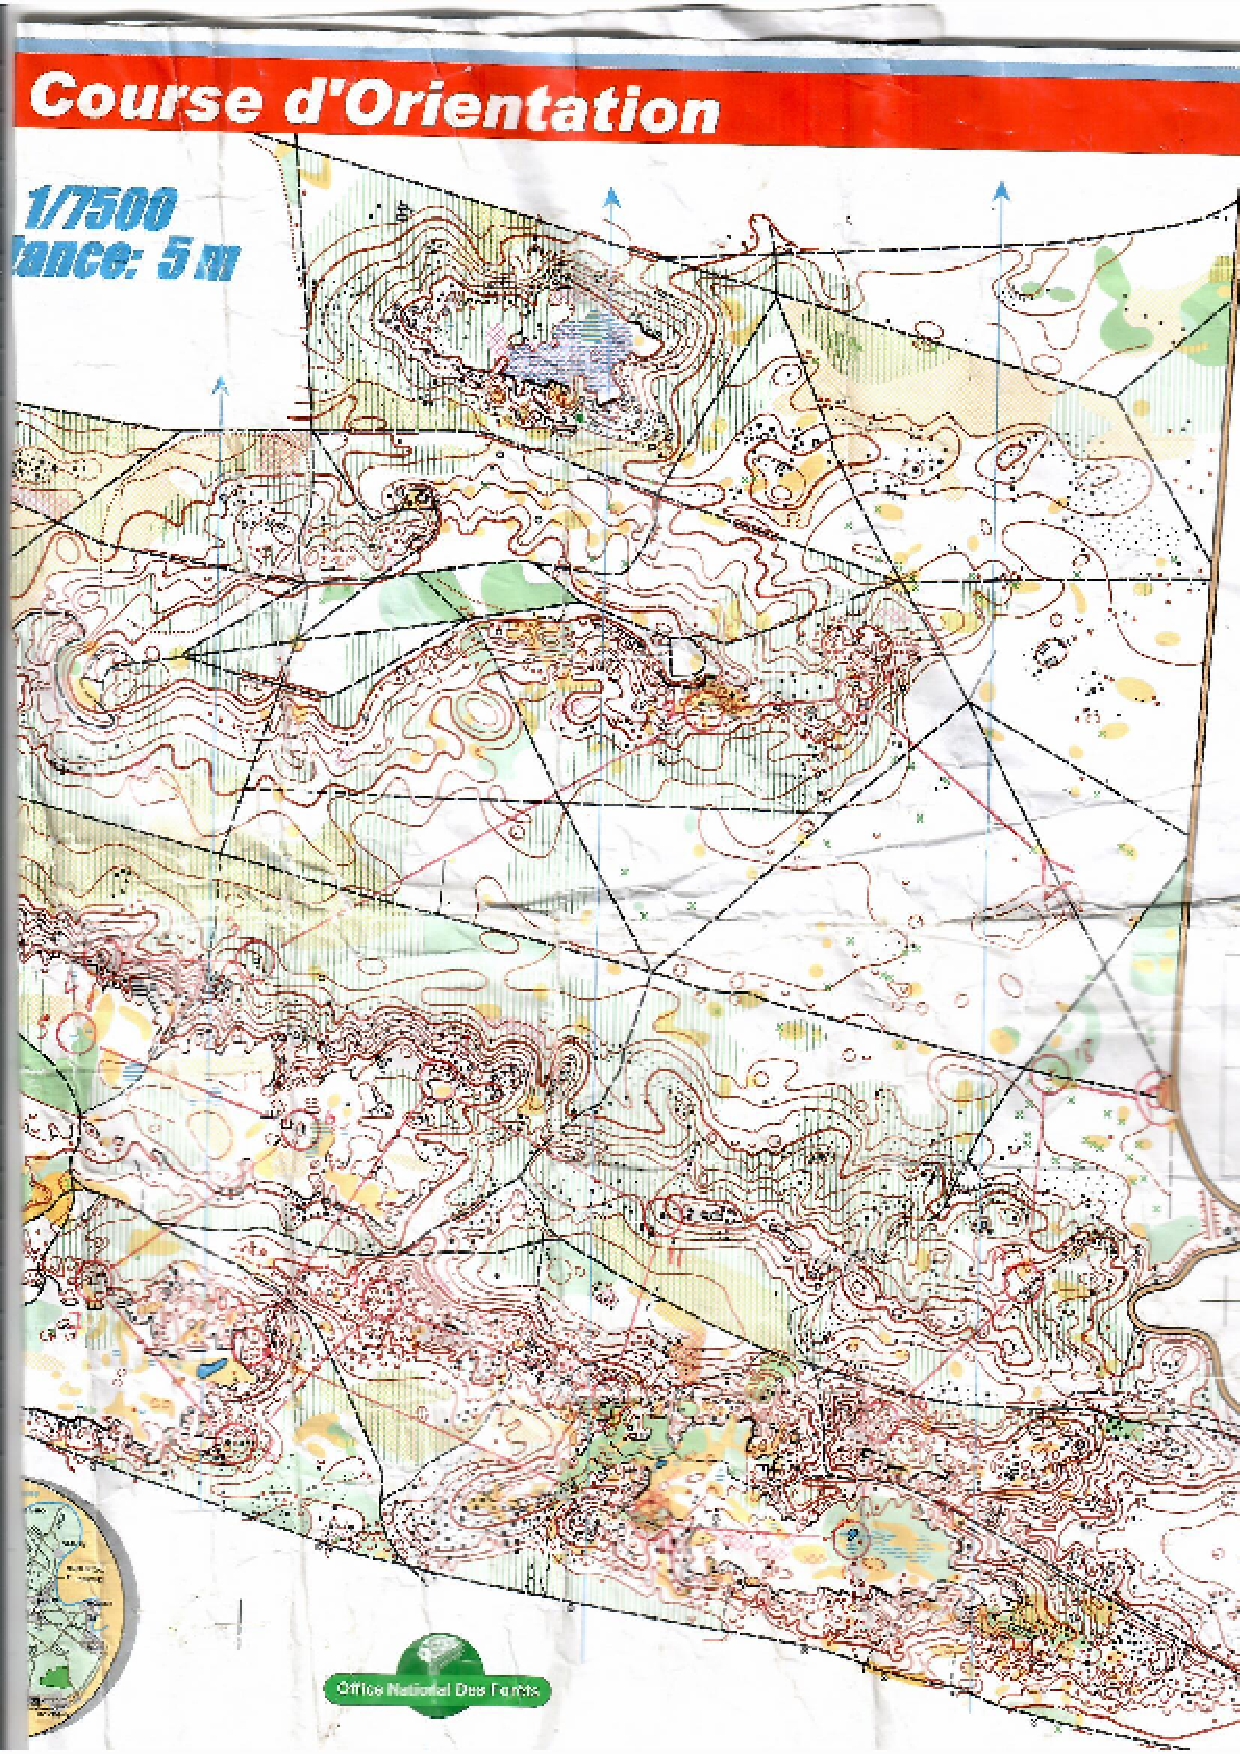
\includegraphics[width=300pt]{le-carrosse.pdf}");
%    B = TEX("\includegraphics[width=300pt]{marly.mps}");

        xmin=3 ;
        xmax=10 ;
        ymin = 1.1 ;
        ymax = 10 ;

        draw A ;
        numeric dx,dy,ratio ;
        dx=0;
        dy=0 ;
        ratio=1 ;
        %draw A ;
%    draw B  scaled ratio shifted (dx,dy);

        fill fullcircle scaled 10 withcolor (1,0,0) ;

        path p ;
        transform t ;
        numeric scale,dx,dy;
        scale=1200;
        dx=10.0cm;
        dy=5.3cm ;
        theta=-5 ;
        t := identity scaled scale rotated theta shifted (dx,dy);
        p := gpx(t) ;

        pair pp[] ;
        pp0 = point 0 of p ;
        fill fullcircle scaled 5 shifted pp0 withcolor (1,0,0);

        pp1 = point 231 of p ;
        fill fullcircle scaled 5 shifted pp1 withcolor (1,0,0);

        pp2 = point 865 of p ;
        fill fullcircle scaled 5 shifted pp2 withcolor (1,0,0);


        pair qq[] ;
        qq0 = (280,160) ;
        fill fullcircle scaled 5 shifted qq0 withcolor (0,0,1);

        qq1 = (54,216) ;
        fill fullcircle scaled 5 shifted qq1 withcolor (0,0,1);

        qq2 = (98,45) ;
        fill fullcircle scaled 5 shifted qq2 withcolor (0,0,1);

        pickup pencircle scaled 1;
        draw p withcolor (0,1,0) ;

        transform tt ;
        qq0 = pp0 transformed tt ;
        qq1 = pp1 transformed tt ;
        qq2 = pp2 transformed tt ;

        path pp ;
        pp = p transformed tt ;
        draw pp withcolor (1,0,0) ;

        path b ;
%    b = bbox B ;
%    draw b withcolor (1,0,0) ;


        endfig;

    \end{mplibcode}

\end{document}
